\chapter{準備}
\section{表記}
整数アルファベットを$\Sigma$とし,$\Sigma$上の全ての系列からなる集合を$\Sigma^\ast$と表し,$\Sigma^\ast$上の要素を文字列と呼ぶ.
文字列$S$の長さを$|S|$と表す.
文字列$S$の$i$番目$(1 \leq i \leq |S|)$の文字を$S[i]$と表し,文字列$S$の$i$番目から$j$番目までの部分文字列を$S[i:j]$と表す.
特に,$1\leq i \leq j \leq |S|$とし,$i > j$の時は空文字列とする.
集合 $L_{[1:m]}$ を,任意の整数 $t$ $(0 \leq t \leq m)$ において,$1 \leq i_1 < \cdots < i_t \leq m$ を満たす添え字列 $I = (i_1, \cdots, i_t) \in \{1, \cdots, m\}^t$ からなる集合とする.
添え字列 $I \in L_{[1:m]}$ において,$I$に対応する文字列$S$の部分列を$S_I = (S[i_1], \cdots, S[i_t])$ と表す.
デカルト木$CT(S)$の根ノードの位置を$CTR(S)$と表す.以下の図\ref{fig:デカルト木}の文字列$S$の場合,$CTR(S)=2$となる.
$TopK(S,k)$を文字列$S$内の要素を値の昇順に並べた時の1番目から$k$番目までの要素に対応する位置からなる集合とする.以下の図\ref{fig:デカルト木}の文字列$S$の場合,$TopK(S,3)=\{2,4,6\}$となる.
\section{デカルト木照合問題}
\begin{definition}[デカルト木~\cite{cartesian-tree}]
  文字列$S[1:m]$に対応したデカルト木$CT(S)$とは以下の規則に従って再帰的に定義される二分木である.
    \begin{displaymath}
      CT(S)=
      \begin{cases}
        \begin{aligned}
          &i \textit{に対応する節点を根,} CT(S[1:i-1]) \text{を左部分木,}\\
          & \qquad CT(S[i+1:m]) \text{を右部分木とした木}
        \end{aligned}&(S \text{は空文字列ではない})\\
        \text{空の木} & (S \text{は空文字列})
      \end{cases}
    \end{displaymath}
    特に,$i$は$S$中の最小値の最左のインデックスである.
\end{definition}

\begin{example}
  文字列$S=(17,10,19,10,24,15,27)$のデカルト木は以下の図\ref{fig:デカルト木}のようになる.
\end{example}

\begin{figure}
  \centering
  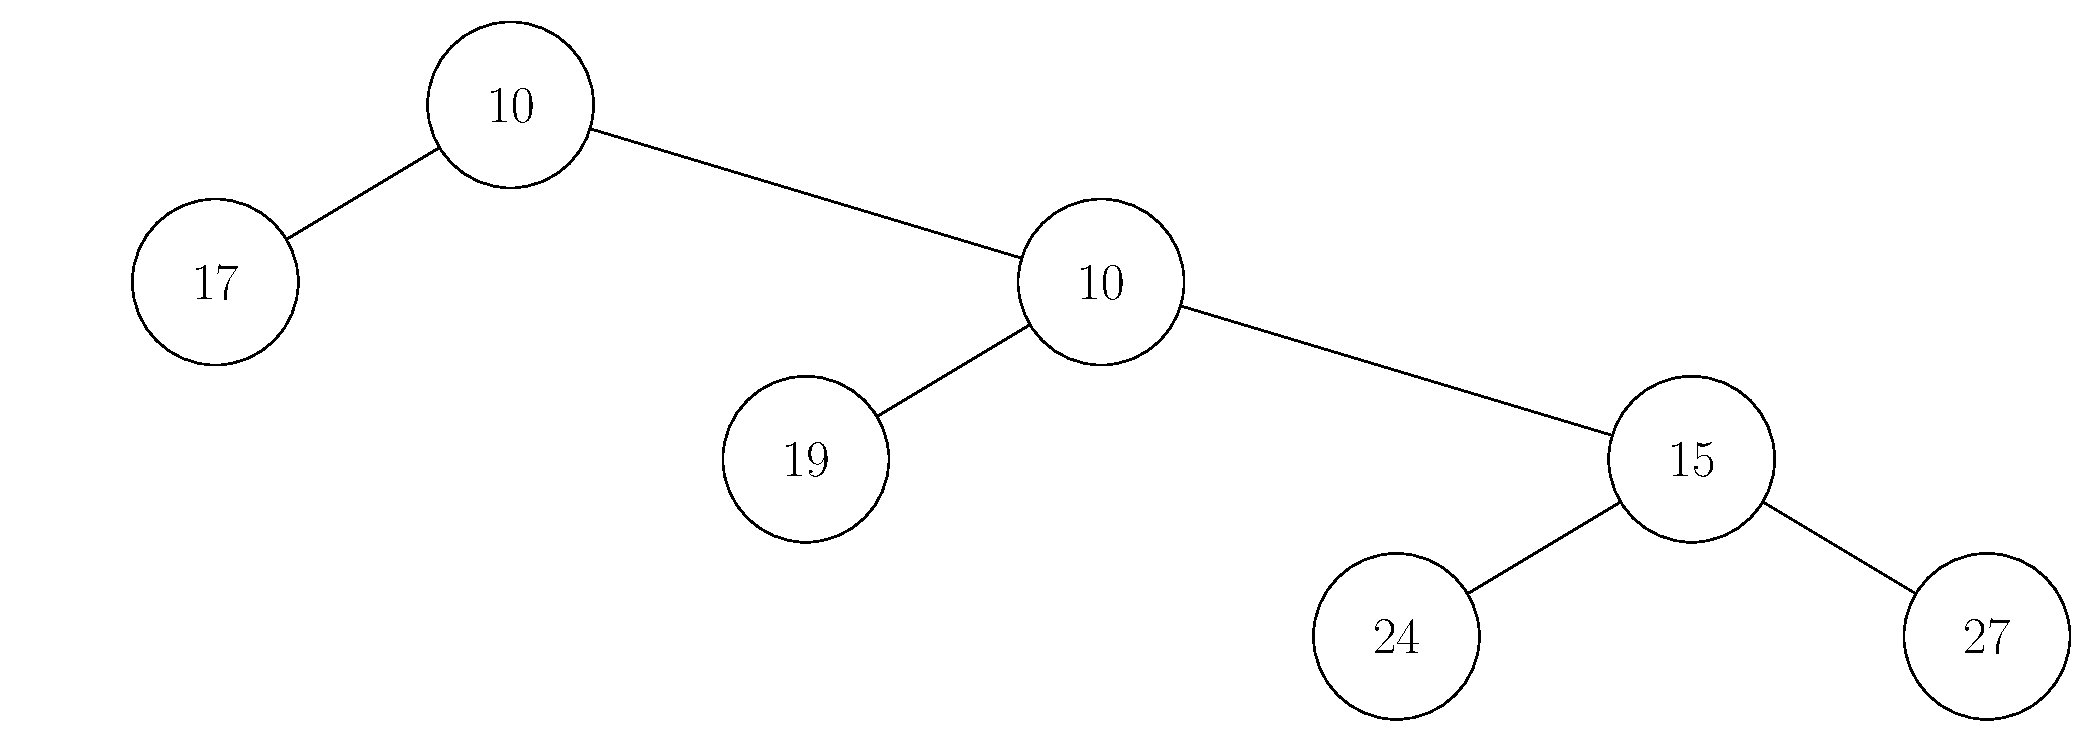
\includegraphics[width=\linewidth]{figs/out/CartesianTree.pdf}
  \caption{文字列$S=(17,10,19,10,24,15,27)$のデカルト木}
  \label{fig:デカルト木}
\end{figure}

\begin{definition}[デカルト木同型]
  同じ長さの文字列$S_1$と$S_2$において,
  \[CT(S_1)=CT(S_2)\]ならば,
  $S_1$と$S_2$はデカルト木同型であると言い,$S_1 \approx S_2$と表記する.
\end{definition}

\begin{definition}[デカルト木照合問題~\cite{cartesian-tree}]
  デカルト木照合問題とは,長さ$n$のテキスト$T$と,長さ$m$のパターン$P$の2つの文字列が与えられた時に,
  \begin{displaymath}
    P[1:m] \approx T[i:i+m-1]
  \end{displaymath}
  を満たす全ての$i\ (1 \leq i \leq n-m+1)$を出力する問題.
\end{definition}

\section{デカルト木ミスマッチ数の定義と問題定義}
同じ長さの文字列$S$と$P$において,$S$と$P$のデカルト木が同型となるための最小のミスマッチ数をデカルト木ミスマッチ数と呼び,以下のように定義する.
\begin{definition}[デカルト木ミスマッチ数]
  長さ$m$の文字列$P$と$S$において,$P$と$S$のデカルト木ミスマッチ数は$CTMiss(S,P)$と書き,以下のように定義される.
  \begin{displaymath}
    CTMiss(S,P)=\min_{I\in L_{[1:m]}}\{m-|I|\mid CT(S_{I})=CT(P_{I})\}
  \end{displaymath}
\end{definition}

\begin{example}
  文字列$P=(17,25,21,11,27,15)$と$S=(21, 60, 30, 40, 50, 10)$において,$CTMiss(S,P)=1$である.
\end{example}

\begin{problem}[$k$ミスマッチデカルト木決定問題]
  同じ長さ$m$の文字列$P$と$S$,許容ミスマッチ数$k\ (0\leq k \leq m)$が与えられた時に,$CTMiss(S,P)\leq k$かどうかを判定する問題.
\end{problem}
